\structure{ОСНОВНАЯ ЧАСТЬ}

\section{Характеристика компании}

\flqq VK Tech\frqq -- это технологическое подразделение крупнейшей российской социальной сети \flqq
ВКонтакте\frqq,
занимающееся разработкой и поддержкой высоконагруженных систем, инструментов для разработчиков, а также
различных продуктоe, поддерживающих экосистему \flqq ВКонтакте\frqq\ и её партнёров. Одним из ключевых направлений
работы \flqq VK Tech\frqq\ является развитие платформы Tarantool.

Tarantool \cite{tarantool} -- это высокопроизводительная платформа, объединяющая в себе функциональность \flqq in-memory\frqq базы
данных и сервера приложений, обеспечивающая низкую задержку и высокую масштабируемость. Tarantool
активно используется как в инфраструктуре «ВКонтакте», так и в других крупных компаниях для обработки
больших объемов данных в реальном времени.

Помимо базового ядра Tarantool, в Enterprise Edition доступны коробочные продукты и решения, которые
закрывают задачи интеграции, масштабирования и эксплуатации:

\begin{itemize}
  \item Tarantool DB -- основной продукт для высоконагруженных OLTP-сценариев, in-memory база данных с
  репликацией и шардингом.
  \item Tarantool CDC (Change Data Capture) —- механизм потоковой передачи изменений из Tarantool во
  внешние системы (Kafka, ClickHouse, PostgreSQL и др.).
  \item Tarantool Queue Enterprise -- система очередей сообщений и задач для надёжного асинхронного обмена,
  с расширенными возможностями мониторинга и отказоустойчивости.
  \item Tarantool Column Store -- колоночное хранилище, ориентированное на аналитические нагрузки.
  \item Tarantool Clusters Federation -- комплекта инструментов для межкластерной репликации данных с
  автоматическим переключением трафика при проблемах на одном кластере.
\end{itemize}

Далее вся информация и объем работы, выполненный в рамках практики, будет относиться к последнему
представленному продукту.

\section{Описание продукта \flqq Tarantool Clusters Federation\frqq}

Tarantool Clusters Federation (TCF) \cite{tcf} позволяет построить отказоустойчивую систему из двух независимых
кластеров Tarantool. В такой системе один из кластеров является активным и принимает все запросы от
приложения. Второй кластер является пассивным и содержит копию данных активного кластера.

TCF позволяет управлять переключением трафика между активным и пассивным кластерами. Например, размещение
кластеров в разных центрах обработки данных позволяет минимизировать негативные последствия при
техногенных или природных инцидентах. Также переключение трафика на другой кластер позволяет проводить
технические работы и изменения логики работы приложения без простоя.

Сам продукт состоит из ролей 

Далее будет представлена подробное описание архитектуры продукта.

На рисунке~\ref{fig:fig01} представлена архитектурная схема для понимания внутреннего устройства системы и взаимосвязей между
ключевыми элементами и участниками.

\begin{figure}
  \centering
  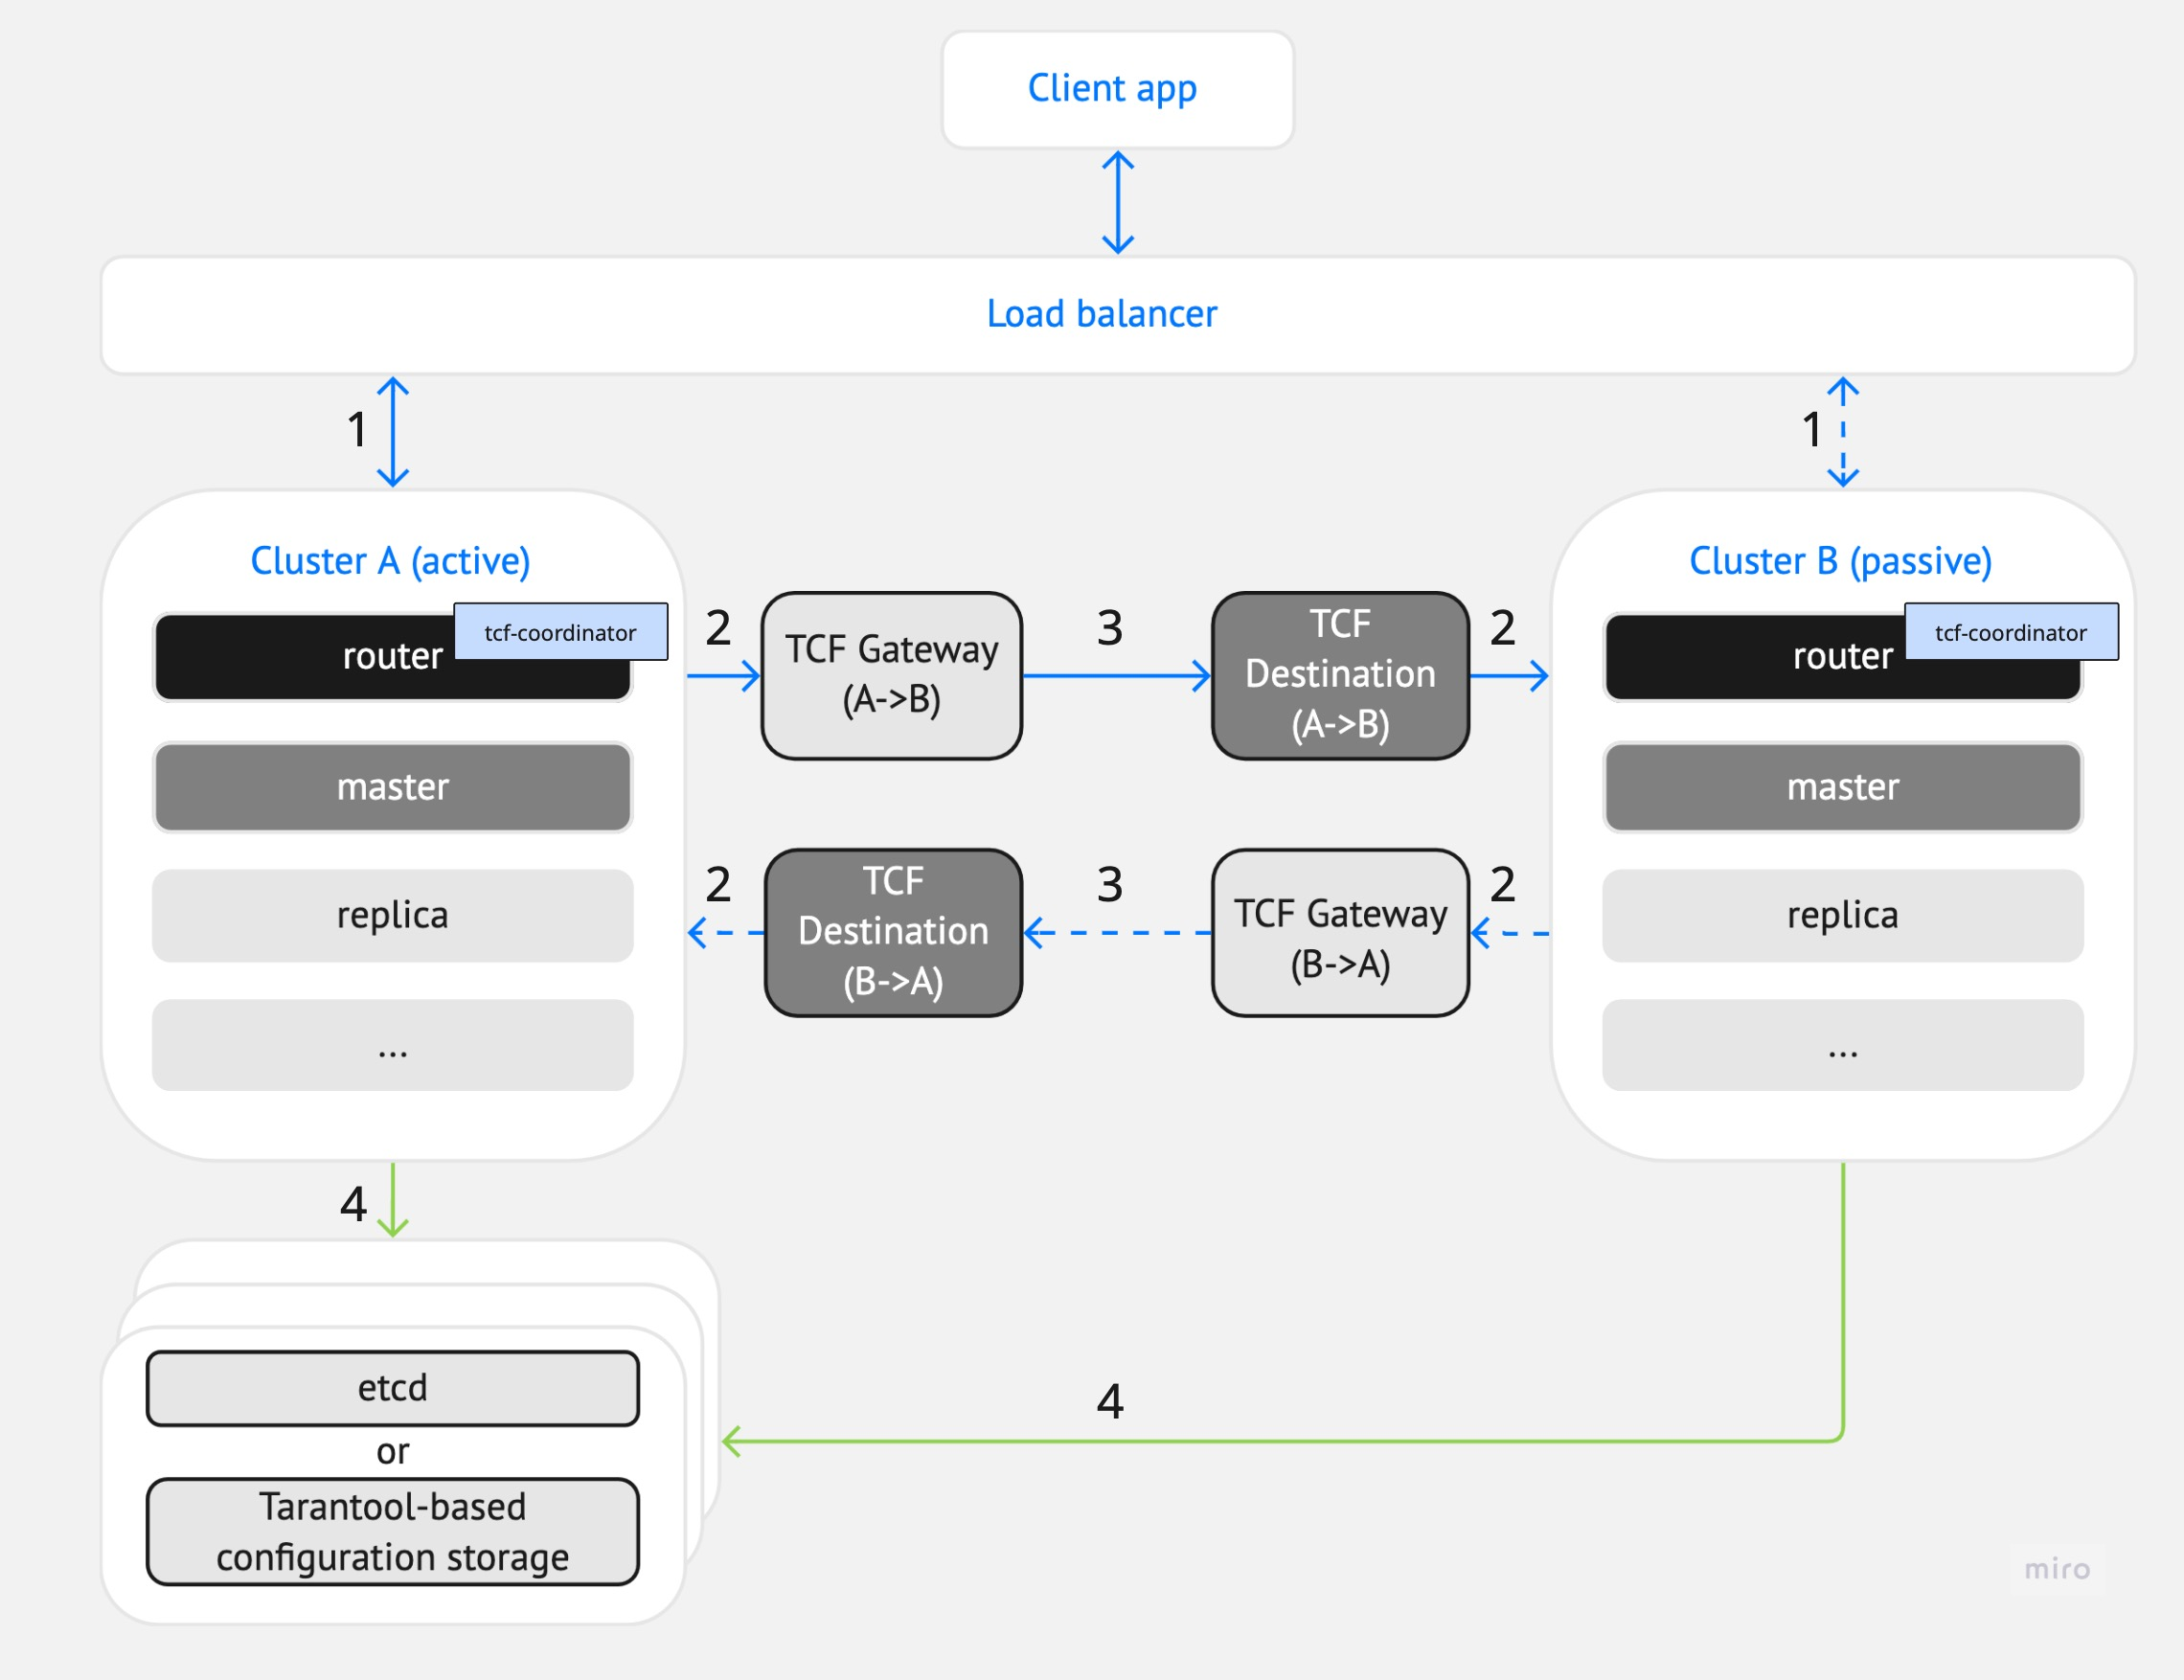
\includegraphics[scale=0.2]{assets/tcf_architecture.jpg}
  \caption{Архитектура взаимодействия компонентов TCF между собой}
  \label{fig:fig01}
\end{figure}

TCF включает следующие компоненты:

\begin{itemize}
  \item Приложение (\textbf{Client app}).
  \item Внешний балансировщик (\textbf{Load balancer}).
  \item Активный и пассивный кластеры (\textbf{Cluster A и Cluster B}).
  \item TCF-координатор в качестве роли на инстансе типа роутер класторв.
  \item TCF-worker в качестве роли на каждом инстансе тарантула.
  \item Репликаторы данных.
  \item Хранилище состояния кластеров (etcd \cite{etcd} или Tarantool-based configuration storage).
\end{itemize}

На рисунке~\ref{fig:fig01} цифрами обозначены элементы и участники взаимодействия в TCF:

\begin{enumerate}[label=\arabic*.]
  \item DML-пользователь. Выполняет DML-операции (чтение, запись, обновление, удаление данных).
  Когда кластер переводится в пассивное состояние, TCF блокирует доступ для всех DML-пользователей данного
  кластера. Таким образом организуется запрет изменения данных на пассивном кластере.
  \item Служебный пользователь репликации данных, который нужен для непосредственной репликации между двумя
  класетрами.
  \item Взаимодействие через gRPC-протокол. В gRPC-конфигурации нет пользователей: в конфигурации Gateway
  указывается адрес для приёма входящих gRPC-запросов от Destination. В конфигурации Destination указывается
  тот же адрес, что и в Gateway, на который компонент отправляет gRPC-запросы. Внешние подключения не
  предполагаются. Разграничение доступа можно обеспечить через TLS и выдачу компонентам сертификатов для
  безопасного взаимодействия друг с другом.
  \item Пользователь хранилища состояния кластеров: etcd или Tarantool-based configuration storage.
\end{enumerate}

Далее будет представлена более подробная информация по каждому из компонентов.

\textbf{Client app} -- приложение, отправляющее запросы на активный кластер Tarantool через внешний балансировщик.
Данное приложение устанавливает соединение с кластером от имени пользователя, у которого есть необходимые
права на чтение и запись в кластер.

\textbf{Load balancer} -- внешний балансировщик, выполняющий переключение трафика между приложением и
кластерами Tarantool. Балансировщик отправляет все запросы на адреса роутеров активного кластера. При
штатной работе трафик от приложения на роутеры пассивного кластера не направляется. Для определения
состояния кластера необходимо отправить HTTP-запрос к любому из узлов кластера на заданный адрес
обработчика запроса.

При активном кластере HTTP-ответ содержит код 200 и строку active. При пассивном — также код 200, но со
строкой passive. При наличии неполадок возможны другие коды ответа из диапазонов 4xx или 5xx.
Балансировщик должен направлять запросы только на активный кластер, то есть на узлы, возвращающие строку
active, и не отправлять запросы на пассивные или неработоспособные кластеры, идентифицируемые по строке
passive или по ошибочным HTTP-кодам.

TCF в типичной конфигурации содержит два идентичных кластера – активный и пассивный:

\begin{itemize}
  \item \textbf{Cluster A} -- активный кластер Tarantool, на который перенаправляются запросы от
  приложения.
  \item \textbf{Cluster B} -- пассивный кластер Tarantool, который содержит копию данных активного
  кластера, но не принимает запросы от приложения.
\end{itemize}

Кластеры хранят свое состояние в централизованном хранилище. Состояние кластеров может быть изменено
вручную или автоматически.

Технологическая роль –- это программный модуль, реализующий определенные функции или логику. Это не те
роли, которые могут быть назначены пользователям. Для работы TCF используются две технологические роли в
конфигурации кластера:

\begin{itemize}
  \item \textbf{TCF-координатор} -- отвечает за автоматическое переключение состояния. Чтобы обеспечить
  отказоустойчивость, в каждом кластере должно быть запущено два и более экземпляра Tarantool с этой ролью.
  Назначается выборочным экземплярам типа storage и router в кластере Tarantool, которыми управляет TCF.
  \item \textbf{TCF-worker} -- инициализирует и координирует переключение статусов кластеров
  (активный-пассивный) и предоставляет базовый HTTP API для управления TCF. Назначается всем экземплярам
  типа storage и router в кластере Tarantool, которыми управляет TCF.
\end{itemize}

Данные с активного кластера на пассивный реплицируются по протоколу gRPC в асинхронном режиме с помощью пары Gateway/Destination (шлюз/приемник):

\begin{itemize}
  \item Gateway подключается к активному кластеру в режиме анонимной реплики для получения потока
  транзакций. Поток транзакций сериализуется в gRPC.
  \item Destination подключается к Gateway по gRPC и запрашивает поток транзакций, затем десериализует
  поток транзакций и записывает их в пассивный кластер по протоколу iproto.
\end{itemize}

На рисунке~\ref{fig:fig01} выше присутствуют две пары Gateway/Destination:

\begin{itemize}
  \item TCF Gateway (A->B) и TCF Destination (A->B): Gateway и Destination, которые используются для
  репликации данных из Cluster A в Cluster B, когда Cluster A является активным;
  \item TCF Gateway (B->A) и TCF Destination (B->A): Gateway и Destination, которые используются для
  репликации из Cluster B в Cluster A, когда Cluster B становится активным.
\end{itemize}

Направление репликации определяется конфигурацией репликаторов данных. Если адреса Gateway/Destination не
указаны в конфигурации, репликация выполняется в обе стороны. Если адреса заданы, переключение кластера в
пассивный режим останавливает соответствующую пару. Односторонняя репликация снижает риск конфликтов,
двусторонняя — компенсирует отставания асинхронной репликации.

Например, в случае сбоев на активном кластере (включая полную временную недоступность), активным
становится текущий пассивный кластер, но из-за асинхронности не гарантируется, что он содержит все
актуальные данные. После восстановления старый активный кластер возвращается в систему как пассивный.
Если в его WAL остались непереданные данные, при двусторонней репликации они будут доставлены на новый
активный кластер; при односторонней — нет, так как пассивный кластер не инициирует передачу данных.

Для работы TCF требуется внешний state provider – централизованное хранилище, которое хранит информацию о
состояниях кластеров.

TCF поддерживает два типа такого хранилища:

\begin{itemize}
  \item etcd -- распределенное хранилище типа ключ-значение;
  \item хранилище конфигурации на основе Tarantool: хранилище, состоящее из набора реплик Tarantool.
\end{itemize}

